\documentclass{report}

% Pacotes para acentuação e formatação

\usepackage[utf8]{inputenc}
\usepackage[T1]{fontenc}
\usepackage[brazil]{babel}
\usepackage{setspace}    % Para espaçamento
\usepackage{lipsum}      % Texto de exemplo (remova se não precisar)
\usepackage{graphicx}
\usepackage{listings}
\renewcommand{\lstlistingname}{Código}


\begin{document}
	
	\begin{titlepage}
		
		\centering
		\vspace*{5cm} % Espaço do topo
		
		{\Huge\bfseries Estrutura de Dados I\par} % Título
		
		\vspace{0.5cm}
		{\Large 2025/2\par} % Ano
		
		\vfill
		{\large Nicolas Ramos Carreira\par} % Nome
		
		\vspace*{2cm}
	\end{titlepage}
	
	\tableofcontents
	\newpage
	
	\chapter{Intuito}
	
	O intuito deste documento é documentar o meu aprendizado da disciplina de estrutura de dados 1. Nesta disciplina começamos estudando sobre a linguagem C até entrar nas principais estruturas de dados. 
	
	\chapter{Fundamentos em C}
	\section{Sobre a linguagem C}
	A linguagem C é uma das linguagens de programação mais influentes e utilizadas da história da computação. Criada na década de 1970 por Dennis Ritchie nos laboratórios Bell, ela foi projetada para ser uma linguagem de propósito geral, eficiente e próxima do hardware, permitindo alto desempenho.
	
	C é considerada uma linguagem de médio nível, pois combina características de linguagens de baixo nível (como manipulação direta de memória) com recursos de alto nível (como funções e estruturas). Sua sintaxe influenciou muitas outras linguagens modernas, como C++, Java, Csharp e até mesmo Python em alguns aspectos.
	
	É amplamente usada em sistemas operacionais, softwares embarcados, drivers e aplicações que exigem alto desempenho. Além disso, aprender C é um ótimo ponto de partida para entender conceitos fundamentais de programação e arquitetura de computadores.
	\section{Estrutura de um programa em C}
		
	\begin{center}
		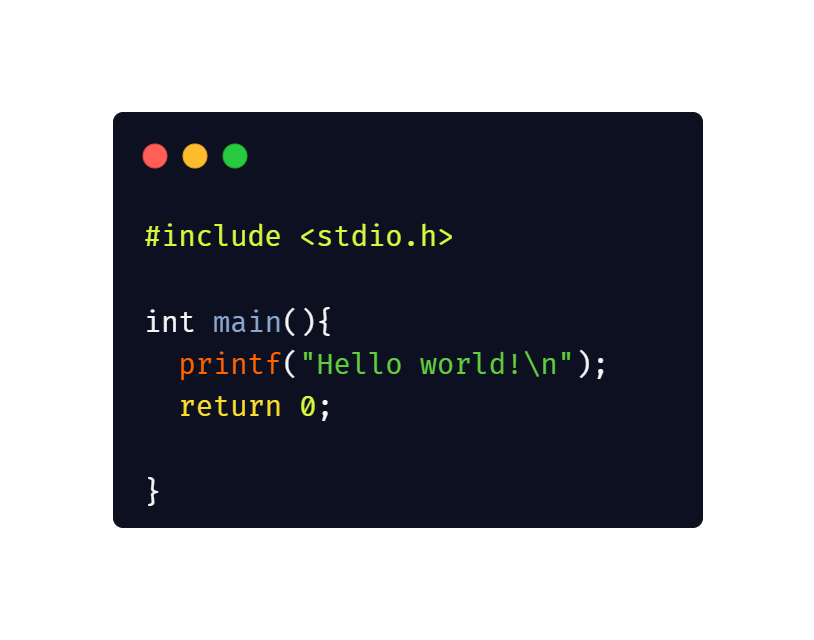
\includegraphics[width=6cm,height=5cm,keepaspectratio=false]{imagens/programac.png}
	\end{center}
	
	A imagem acima mostra um programinha extremamente simples em C, um Hello, world. Para iniciar um programa em C, nós sempre começamos declarando a biblioteca principal, que é a stdio.h (poderíamos ter outras bibliotecas inclusive, mas essa é a principal e DEVE estar lá). 
	
	Depois disso, nós declaramos o local do programa principal, onde fazemos o programa em si. 
	
	Um detalhe é que ao final de cada coisa SEMPRE temos que ter o ponto e vírgula (;), pois se não o nosso programa não compila.
	
	\section{Aspectos da linguagem C}
	\subsection{Variaveis}
	\subsubsection{O que são e pra que são usadas}
	Varivel, em linguagens de programação, é basicamente uma posição alocada da memória para guardar uma informação. Variaveis podem ser modificadas pelo programa e devem ser definidas antes de ser utilizadas
	\subsubsection{Declaração de variaveis em C}
    Para definir variaveis em C, nós precisamos passar o tipo de dado e nome da variavel, no formato: 
    
    \begin{LARGE}
    	\begin{center}
    		<tipo de dado> nome-da-variavel;
    		
    	\end{center}
    \end{LARGE}

    \begin{description}
     	\item[Obs:] ao fazer da forma acima, estamos apenas declarando a variavel, sem atribuir um valor a ela
     \end{description}
    
    O tipo de dado deve ser aqueles que são aceitos pela linguagem (inteiro, decimais, caracteres, booleanos..), mas como falaremos sobre tipos de dados mais pra frente, não entraremos em detalhes agora. O nome da variavel é algo bem importante a se considerar, pois existem algumas regras e boas práticas importantes quanto a isso:
    \begin{itemize}
    	\item Nomes de variaveis devem iniciar com letras ou underscore 
    	\item Os caracteres da variavel devem ser letras, numeros ou underscore (não utilizar acentos ou simbolos)
    	\item Não utilizar espaço em nomes de variaveis
    	\item Palavras chaves (palavras que são reservadas pela linguagem para fazer determinadas coisas) não podem ser usadas como nomes 
    	\item Letras maiusculas e minusculas são consideradas diferentes
    \end{itemize}
    
    Só para deixar totalmente claro, as palavras chaves que a linguagem C usa são:
    
    \begin{figure}[ht]
    	\centering
    	% ajusta a largura da imagem para ser quadrada (ex: 5cm x 5cm)
    	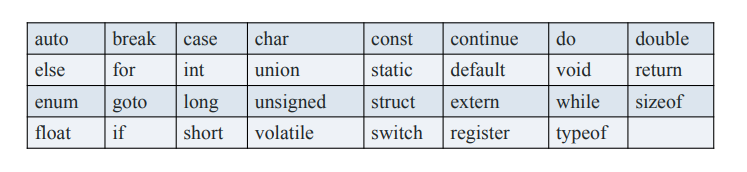
\includegraphics[width=9cm,height=2cm,keepaspectratio=false]{imagens/reservadas.png}
  
    \end{figure}
    
    \subsubsection{Atribuição de valores em variaveis}
    
    Tendo o formato <tipo de dado> nome-da-variavel, podemos atribuir valores a elas (ou seja, armazenar valores dentro da memória). Para isso, basta fazer:
    
    \begin{LARGE}
    	\begin{center}
    		<tipo de dados> nome-variavel = valor;
    	\end{center}
    \end{LARGE}
    
	\subsection{Tipos de dados}
	Como falamos anteriormente na parte de variaveis, quando vamos defini-las, nós temos que declarar o tipo de dado da variavel. O tipo de dado define os valores que aquela variavel pode assumir e as operações que podem ser realizadas com ela.
	Os tipos de dados principais são: char, int, float e double
	\subsubsection{Char}
	Um byte que armazena
	\subsubsection{Int}
	Um inteiro cujo o tamanho do numero que pode ser alcançado depende do processador (tipicamente 16 ou 32 bits)
	\subsubsection{Float}
	Basicamente numeros decimais com precisão simples (em C a parte decimal usa ponto e não vírgula)
	\subsubsection{Double}
	Também números decimais, mas com precisão dupla. É usados para numeros muito pequenos (cientificos por exemplos) ou muito grandes
	
	\subsubsection{Bool}
	Esse tipo de dados é muito interessante, pois ele pode assumir dois valores: verdadeiro ou false (true ou false). Em outras linguagens, nós temos literalmente um valor True e False. No entanto, na linguagem C nós não temos True e False, mas podemos representá-los como 1 e 0, respectivamente.
	\subsubsection{Outros tipos}
	Na imagem abaixo, você poderá ver alguns outros que são utilizados:
 	\begin{center}
		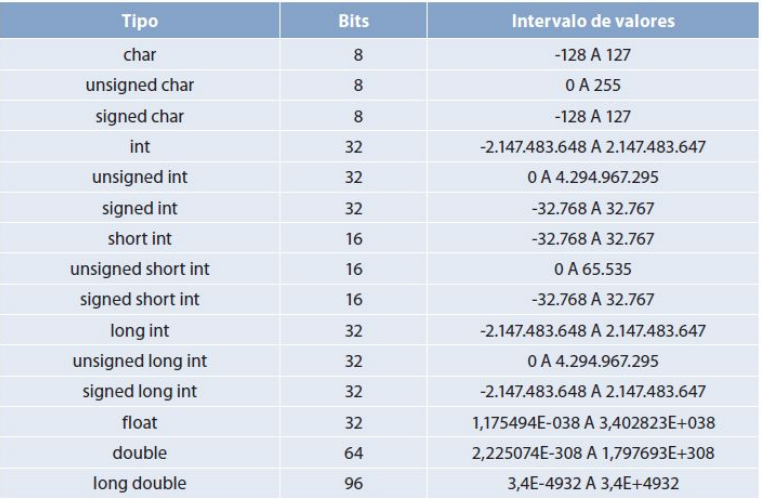
\includegraphics[width=8cm,height=7cm,keepaspectratio=false]{imagens/tipos.png}
	
	\end{center}
	
	\subsection{Input e output}
	Input e output é basicamente a entrada e a saída de dados. As vezes, podemos querer receber do usuário alguns valores, para fazer alguma coisa com eles e depois entregá-los com modificações. É basicamente isso. Um detalhe é que para o output, não necessariamente nós precisamos ter recebido algo.
	\subsubsection{Especificadores de formato}
	\subsubsection{Saída com printf()}
	Vamos começar com a saída de dados. Para exibir algo na tela. Fazemos:
	\begin{figure}[ht]
		\centering
		% ajusta a largura da imagem para ser quadrada (ex: 5cm x 5cm)
		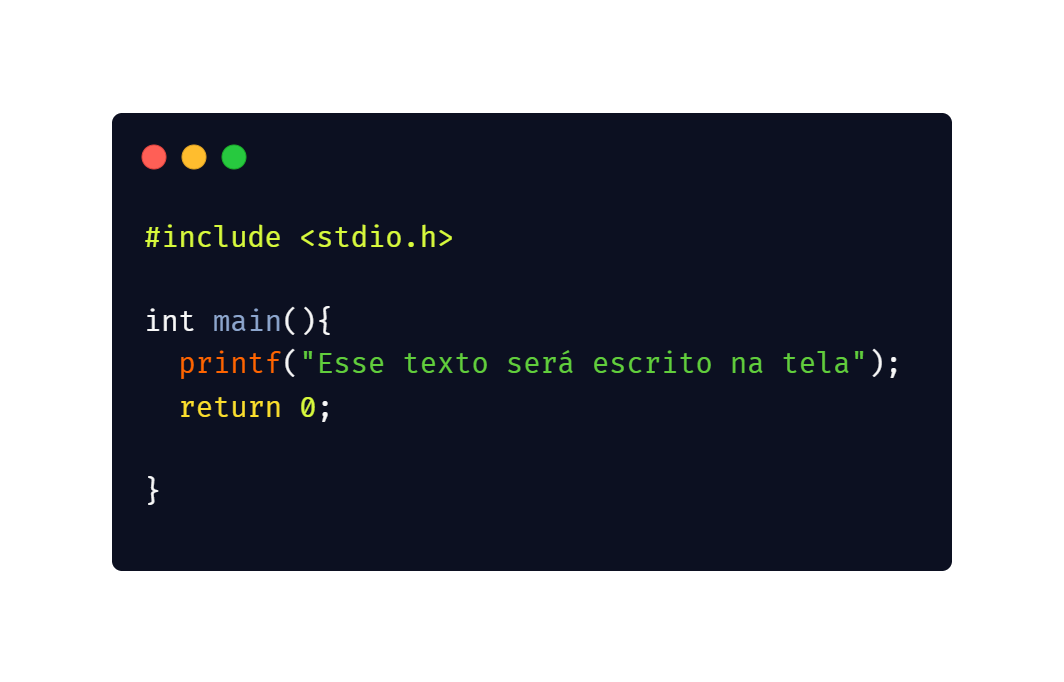
\includegraphics[width=6cm,height=3cm,keepaspectratio=false]{imagens/print.png}
		
	\end{figure}
	
	Ao fazer isso, em nosso terminal será exibido o texto que digitamos dentro do printf ("Esse texto será escrito na tela). Veja:
	
	\begin{center}
		
		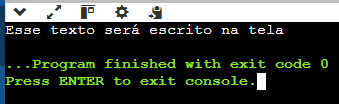
\includegraphics[width=7cm,height=2cm,keepaspectratio=false]{imagens/outputc.png}
	\end{center}
	
	\subsubsection{Uso do escape no printf()}
	Um detalhe é que algo que podemos utiliza no printf é caracter de escape . Esse caracter é utilizado sempre ao final do que que queremos escrever na saída e ele serve para quebrar a linha após a saída. Veja:
	
	\begin{figure}[ht]
		\centering
		% ajusta a largura da imagem para ser quadrada (ex: 5cm x 5cm)
		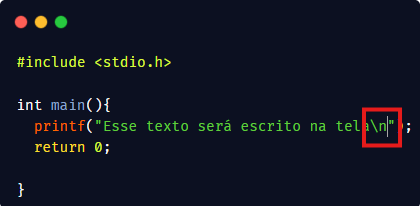
\includegraphics[width=6cm,height=3cm,keepaspectratio=false]{imagens/escape.png}
		
	\end{figure}
	
	
	Se fizermos vários printf, por exemplo, e não usarmos o caracter de escape em nenhum deles, o que escrevemos nos prints, ficará tudo junto. Veja:
	
	\begin{figure}[ht]
		\centering
		% ajusta a largura da imagem para ser quadrada (ex: 5cm x 5cm)
		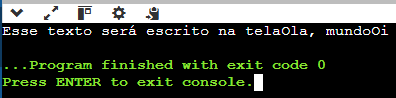
\includegraphics[width=6cm,height=3cm,keepaspectratio=false]{imagens/noescape.png}
	\end{figure}
	
	\subsubsection{Exibindo valores de variaveis no output}
	Se quisermos que em nosso output seja usada alguma variavel, temos que utilizar o seguinte formato:
	
	\begin{figure}[ht]
		\centering
		% ajusta a largura da imagem para ser quadrada (ex: 5cm x 5cm)
		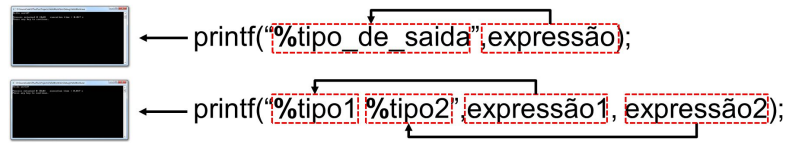
\includegraphics[width=9cm,height=2cm,keepaspectratio=false]{imagens/tipo_saida.png}
	\end{figure}
	
	Isso acima significa que se quisermos passar no output uma variavel que tenha o tipo int, nós teríamos que passar o tipo de saida  dentro das aspas duplas e depois separar por virgula passando a nossa variavel. Mas você deve estar se perguntando: Como assim tipos de saida? Veja abaixo os tipos de saida que usaremos no output (printf):
	
	\begin{center}

		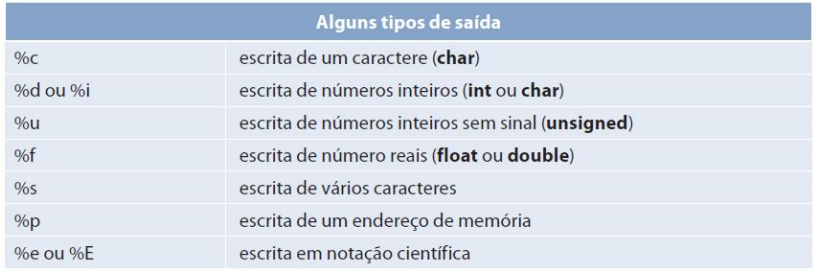
\includegraphics[width=8cm,height=3cm,keepaspectratio=false]{imagens/comando_saida.png}
	\end{center}
	
	Ou seja, seguindo o exemplo da variavel de tipo int que tinhamos dado, se quiséssemos exibi-la no output (printf), faríamos:
	
	\begin{LARGE}
		\begin{center}
			printf("porcentagemd", variavel);
		\end{center}
	\end{LARGE}
	
	\subsubsection{Entrada com scanf()}
	Agora, falando sobre entrada de dados, o comando que utilizamos para passar dados para o nosso programa é o scanf(). Esse comando permite realizar a leitura de dados da entrada padrão (teclado). Sua estrutura é a seguinte:
	
	\begin{center}
		
		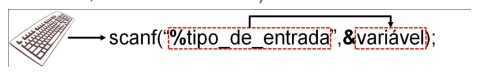
\includegraphics[width=7cm,height=2cm,keepaspectratio=false]{imagens/inputar.png}
	\end{center}
	
	Sendo que, os tipos de entrada são praticamente os mesmos que vimos nos tipos de saida. Veja:
	
	\begin{center}
		
		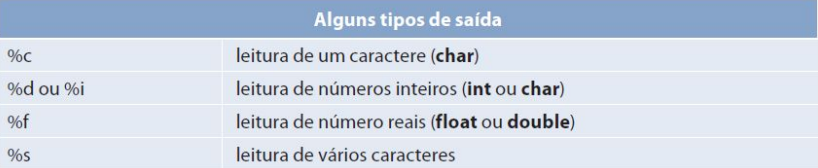
\includegraphics[width=7cm,height=2cm,keepaspectratio=false]{imagens/tipos_entrada.png}
	\end{center}
	
	Podemos ainda realizar a leitura de mais de um valor (assim como podemos fazer o output de mais de um valor). É bem parecido com o output também. Veja:
	
	
	\begin{center}
		
		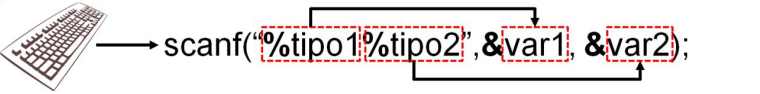
\includegraphics[width=7cm,height=2cm,keepaspectratio=false]{imagens/inputar_varios.png}
	\end{center}
	
	
	\subsection{Contantes}
	Assim como variaveis, constantes também armazenam um valor na memória do computador. A principal diferença para as variaveis é que esse valor não será alterado. Outra coisa é que para as constantes é obrigatoria a atribuição de valor, diferente das variaveis que podemos simplesmente declará-las sem dar um valor
	\subsubsection{Declaração de constantes}
	Para declarar uma constante existem duas formas. Na primeira, devemos  utilizar define nome-costante <valor> no começo do programa. Uma detalhe é que neste caso, não usaremos ponto e virgula no final. Veja:
	
	\begin{center}
		
		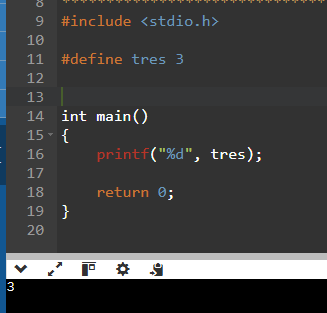
\includegraphics[width=5cm,height=4cm,keepaspectratio=false]{imagens/define.png}
	\end{center}
	
	Outra forma é fazer: const <tipo> nome = valor;. Como você pôde ver, nesse caso, temos que usar o ponto e vírgula. Veja:
	
	\begin{center}
	
	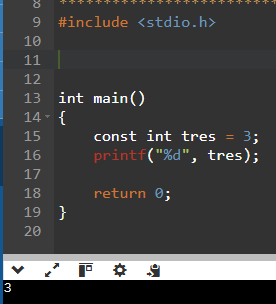
\includegraphics[width=5cm,height=4cm,keepaspectratio=false]{imagens/const.png}
	\end{center}	
	
	\subsubsection{Curiosidade sobre constantes}
	Já chegamos a falar sobre caracteres de escape (no caso, falamos apenas do barran). Os caracteres de escape são constantes pre-definidas. Veja cada um deles:
	
	\begin{center}
		
		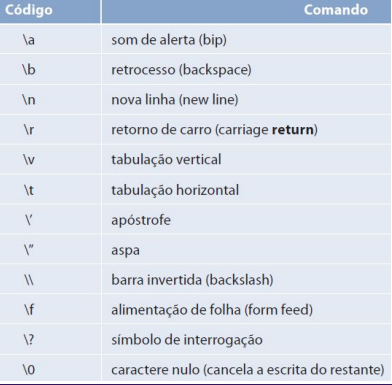
\includegraphics[width=7cm,height=6cm,keepaspectratio=false]{imagens/outros_escape.png}
		
	\end{center}
	
	
	\subsection{Operadores}
	Os operadores são usados para desenvolver diferentes tipos de operações. Com eles podemos fazer operações matematicas, comparativas, logicas e etc. Veremos acerca de cada um dos operadores a seguir
	\subsubsection{Operadores aritméticos}
	Os operadores aritméticos são aqueles que operam sobre numeros e/ou sobre expressões que tem como resultado valores numéricos. Veja os operadores:
	
	\begin{center}
		
		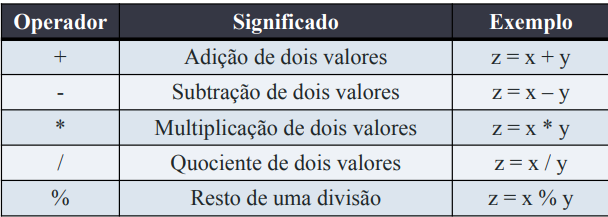
\includegraphics[width=6cm,height=3cm,keepaspectratio=false]{imagens/operadoresa.png}
		
	\end{center}
	
	Um detalhe é que as operações seguem a mesma ordem da matemática. A prioridade são as operações de multiplicação e divisão em detrimento das de soma e subtração.
	
	Outro detalhe é que na divisão, se o numerador e denominador forem inteiros, o compilador retornará apenas a parte inteira da divisão
	
	\subsubsection{Operadores relacionais}
	São aqueles que verificam a magnitude (maior/menor) e/ou igualdades entre dois valores e/ou expressões. Esses operadores retornam verdadeiro (1) ou falso (0) (ou seja, um valor booleano). Veja cada um deles:
	
	\begin{center}
		
		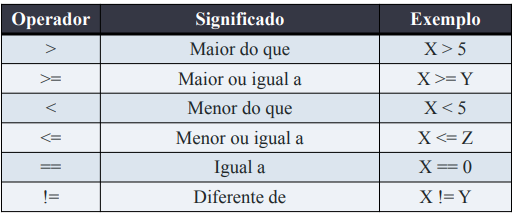
\includegraphics[width=6cm,height=3cm,keepaspectratio=false]{imagens/relacionais.png}
		
	\end{center}
	
	
	\subsubsection{Operadores lógicos}
	
	Os operadores lógicos nos permitem representar situações lógicas unindo duas mais expressões relacionais simples em uma composta e nos retornam verdadeiro (1) ou falso (0). Veja cada um deles:
	
	\begin{center}
		
		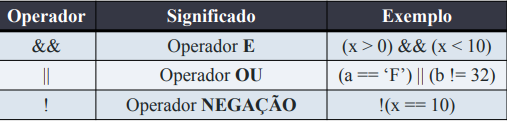
\includegraphics[width=7cm,height=2cm,keepaspectratio=false]{imagens/logicos.png}
		
	\end{center}
	
	\subsubsection{Operadores de atribuição simplificada}
	Muitas vezes em nosso código nós temos que atribuir valores a nossa variavel. Uma forma de fazer isso de maneira mais fácil é utilizando os operadores de atribuição simplificada. Com eles, podemos adicionar valores a nossa variavel de forma muito mais simples. Veja cada um deles:
	
	\begin{center}
		
		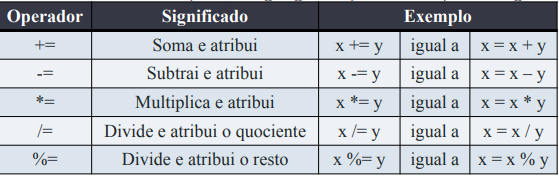
\includegraphics[width=7cm,height=2cm,keepaspectratio=false]{imagens/operadoresatribuicaosimp.png}
		
	\end{center}
	
	
	\subsubsection{Operadores de pré e pós incremento}
	Esses operadores podem ser utilizados sempre que for necessário somar uma unidade (incremento) ou subtrair uma unidade (decremento) a determinado valor. Veja cada um deles:
	
	\begin{center}
		
		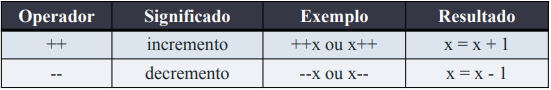
\includegraphics[width=8cm,height=2cm,keepaspectratio=false]{imagens/pospre.png}
		
	\end{center}
	
	Um detalhe é que como você pode ver na imagem acima, podemos utilizar o operador antes de depois da variavel, mas qual a diferença? Veja abaixo:
	
	\begin{center}
		
		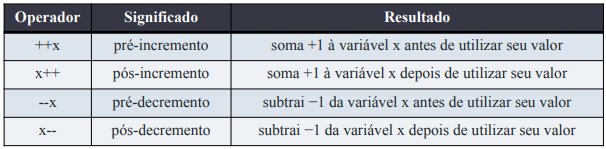
\includegraphics[width=8cm,height=3cm,keepaspectratio=false]{imagens/expliqprepos.png}
		
	\end{center}
	
	\subsection{Coerção de tipos}
	Lembra quando falamos anteriormente que se dividirmos um numero inteiro por outro inteiro seu resultado sempre será inteiro, desconsiderando assim a parte decimal? Podemos contornar isso utilizando o casting. O casting é aplicado sobre uma expressão aritmética e força o resultado da expressão a ser de um tipo especificado. Veja as diferentes formas de utilizar o casting:
	
		
	
	\subsubsection{Type casting explicito}
	Nós faremos a conversão de tipo no resultado da expressão:
	
	\begin{center}
		
		\begin{lstlisting}{caption=casting explicito em C, language=C, label=clanguage}
	int a = 5, b = 2;
	float resultado = (float)a / b;
	printf("%f\n", resultado);  // saida: 2.500000
			
			
		\end{lstlisting}
	\end{center}
	
	\subsubsection{Type casting nos operandos}
	Faremos o casting nos dois operandos da operação para obter o resultado no tipo que queremos
	
	\begin{center}
		
		\begin{lstlisting}{caption=casting explicito em C, language=C, label=clanguage}
	double resultado = (double)a / (double)b;
	printf("%lf\n", resultado); // saida: 2.500000

			
			
		\end{lstlisting}
	\end{center}
	
	\subsection{Condicionais}
	Certo. Agora falaremos sobre condicionais. Condicional é basicamente uma mudança de fluxo em nosso código. Caso uma determinada expressão atenda determinada condição, nosso código seguirá por um fluxo e caso contrário, seguirá para outro fluxo. Existem diferentes maneiras de se utilizar as condicionais em nosso código. Veremos cada uma delas abaixo.
	\subsubsection{If-else}
	A estrutura do if-else é feita da seguinte forma em nosso código:
	
	\begin{center}
		
		\begin{lstlisting}{caption=casting explicito em C, language=C, label=clanguage}
	if(condicao){
		sequencia de comandos 1;
	}
	else{
		sequencia de comandos 2;
	}
			
		\end{lstlisting}
	\end{center}
	
	
	O que acontece acima é que se a condição for satisfeita, ou seja, for verdadeira (tiver valor 1), nosso programa entrará nesse fluxo e executará o código dentro da condição. Caso contrário, ou seja, caso a condição não for satisfeita (for falsa (ter valor 0)), entraremos no fluxo do else.
	
	Um detalhe é que alem do if e do else, podemos ter ainda o else if, onde caso a condição do if não for satisfeita, haverá a condiçao do else if a ser satisfeita e aí se ela não satisfeita também, iremos para o else. Veja:
	
	\begin{center}
		
		\begin{lstlisting}{caption=casting explicito em C, language=C, label=clanguage}
	if(condicao){
		sequencia de comandos 1;
	}
	else if(condicao){
		sequencia de comandos 2;
	}
	else{
		sequencia de comandos 3;
	}
			
		\end{lstlisting}
	\end{center}
	
	\subsubsection{Swicth-case}
	O switch-case é outra estrutura de controle de fluxo de código. Sua estrutura é a seguinte:
	
	\begin{center}
		
		\begin{lstlisting}{caption=casting explicito em C, language=C, label=clanguage}
	switch(expressao){
		case valor 1:
			sequencia de comandos 1;
			break;
		
		case valor k:
			sequencia de comandos k;
			break;
		...
		default:
			sequencia de comandos padrao;
			break;
		
			
		\end{lstlisting}
	\end{center}
	
	O o switch, como podemos ver acima é próprio para testar uma variavel em relação a diversos valores pré-estabelecidos. Além disso, como podemos ver acima o default irá desempenhar o valor que o else desempenha na estrutura if-else
	\subsection{Loops}
	Agora falando sobre loops, o nome já entrega. Os loops serão responsáveis por repetir um bloco de código a partir de uma condição. Enquanto a condição for verdadeira, o bloco de código permanecerá se repetindo. Existem diferentes tipos de loops. Vamos a cada um deles.
	
	\subsubsection{While}
	\subsubsection{Do-While}
	\subsubsection{For}
	\subsection{Arrays}
	Quando vimos sobre variaveis, estudamos que elas podem armazenar um valor. Sempre que tentamos armazenar um novo valor dentro da variavel o antigo valor é sobrescrito (e portanto, perdido). Agora, pense: E se quisessemos armazenar mais de um valor em uma variavel? Para isso, usamos os arrays, que é basicamente uma sequencia de elementos do mesmo tipo, onde cada elemento é identificado por um indice. Ou seja, quando criamos um array, nós alocamos um espaço na memória (onde, quanto maior o tamanho do array, que é a quantidade de elementos que ele pode armazenar, maior o espaço de memoria alocado) e podemos armazenar dentro dele varios valores do mesmo tipo (os valores podem ser acessados por meio do indice do elemento dentro do array, que é basicamente a posição do elemento lá dentro). Um exemplo que pode fazer você entender melhor é: suponhamos que queiramos armazenar em um local a nota de 5 alunos. Para isso, poderiamos usar um array.
	\subsubsection{Declaração de arrays}
	Para declarar um array, nós fazemos da seguinte forma:
	
	\begin{LARGE}
		\begin{center}
			<tipo-array> nome-array[tamanho];
		\end{center}
	\end{LARGE}
	
	Ou seja, primeiro nós precisamos declarar o tipo do array, que será o tipo dos valores que aquele array irá armazenar, depois passamos o nome do array e depois passamos o tamanho do array, ou seja, a quantidade de elementos que ele poderá armazenar.
	
	
	
	\subsubsection{Inserindo e acessando valores dentro de arrays}
	Com o array declarado, caso quisermos inserir algum valor no array, basta fazer: 
	
	\begin{LARGE}
		\begin{center}
			nome-array[indice] = valor;
		\end{center}
	\end{LARGE}
	Lembrando que o indice é a posição do elemento dentro do array. Se tivessemos um array de tamanho 10 e quisessemos inserir um valor no sexto elemento, faríamos: nome-array[5] = valor; (uma vez que os indices começariam do 0 e iriam até o 9).
	
	Para acessar valores de um array, basta fazer:
	
	
	\begin{LARGE}
		\begin{center}
			nome-array[indice];
		\end{center}
	\end{LARGE}
	
	
	\subsubsection{Observações}
	Em C e C++, se tivermos um array que pode armazenar 10 elementos e tentarmos armazenar 11 elementos, o elemento que sobrar irá ser armazenado em um espaço da memória que não pertence ao array, o que causa comportamento indefinido (pode sobrescrever dados, travar o programa e entre outros)
	
	Outro detalhe é que se tivermos um array de 10 elementos (ou seja, teremos 10 indices, do 0 ao 9) e tentarmos acessar o indice 10 (11º elemento) o que acontecerá (em C e C++) é que iremos acessar um elemento da memória que não pertence oficialmente ao array, o que pode retornar "Lixos de memória".
	
	
	\subsection{Struct - Criação de tipos}
	Agora, falaremos sobre structs, estamos falando de uma composição de variaveis de outros tipos que formam um "novo tipo de dado". Assim como temos o tipo inteiro, float e etc, podemos "criar" um outro tipo que será um agrupamento de dados.
	\subsubsection{Declaração}
	
	\subsubsection{Inserindo valores e acessando valores}
	
	\subsection{Comando typedef}
	O comando typedef nos permite "dar um alias" para os tipos de dados existentes na linguagem C. Se temos, por exemplo, o tipo float, mas queremos que ele se chame flutuante, poderíamos fazer isso. 
	\subsubsection{Como usar}
	Para usar, basta fazer o seguinte:
	
	\begin{LARGE}
		\begin{center}
			typedef <tipo-de-dado> <alias>;
		\end{center}
	\end{LARGE}
	
	O comando acima "da um alias" a um tipo de dado existente. Um detalhe é que o comando acima deve estar no topo do programa, juntamente com a inclusão das bibliotecas.
	
	\subsubsection{Exemplo}
	
	\chapter{Acerca de ponteiros}
	\section{O porquê de estudar esse topico}
	Agora, iniciaremos um tópico mais avançado, que são os ponteiros. É muito importante entendermos sobre esse conceito porque várias das estruturas de dados que aprenderemos nesta disciplina dependem deles (listas, pilhas, filas, árvores e grafos), então sem entender isso, não iremos para frente
	\section{O que são e como usá-los}
	\subsection{O que é}
	Conceitualmente, um ponteiro é uma variavel que armazena o endereço de memoria de outra variavel. Ou seja, diferentemente das variaveis comuns, um ponteiro não irá armazenar um valor como um caracter, por exemplo, mas sim, um endereço de memória.	
	\subsection{Declaração de ponteiros}
	Para criar um ponteiro, a estrutura lembra bastante a forma como nós criamos as variaveis, mas com pequenas mudanças. Veja como declaramos um ponteiro:
	
	\begin{LARGE}
		\begin{center}
			<tipo de dado> *nome ponteiro;
		\end{center}
	\end{LARGE}
	
	Perceba que para declarar um ponteiro, assim como nas variaveis, nós temos que usar um tipo de dado. Isso acontece porque nós estamos indicando para o ponteiro que estamos criando o tipo de dado do lugar da memória que ele vai apontar. Isso é importante porque não é muito aconcelhavel você ter um ponteiro inteiro e apontar para um char, por exemplo.
	
	Um detalhe é que podemos criar o nosso ponteiro apontando ele para NULL, para que ele não aponte para nenhum lugar (para que consigamos administrar para onde ele aponta depois). Fazendo isso, a declaração ficaria:
	
	\begin{LARGE}
		\begin{center}
			<tipo de dado> *nome ponteiro = NULL;
		\end{center}
	\end{LARGE}
	
	Se não declararmos da maneira acima e utilizarmos a primeira versão de declaração (<tipo de dado> *nome ponteiro;), o que acontece é que nosso ponteiro irá apontar para um endereço de memória aletório.
	
	Um outro detalhe bem interessante é que podemos fazer com que nosso ponteiro aponte para o endereço de memória de uma variavel já existente. Veja:
	
	\begin{LARGE}
		\begin{center}
			<tipo de dado> *nome ponteiro = a;
		\end{center}
	\end{LARGE}
	
	
	Ou seja, o endereço de memória que nosso ponteiro irá apontar, será o endereço da variavel a (esse  significa que estamos nos referindo ao endereço de memoria da variavel a. Desta forma, o ponteiro b apontará para o endereço de memoria de a).
	
	\subsection{Detalhe após a declaração}
	
	Quando declaramos um ponteiro(exemplo: int *a), algo importante de se dizer é que se utilizarmos *a em qualquer outro trecho do nosso código, nós não vamos estar usando o ponteiro em si, mas sim o valor que está no endereço apontado pelo ponteiro a. Veja um exemplo:
	
	
	\subsection{Exemplo de uso}
	Veja abaixo um exemplo de uso de ponteiros:
	
	\begin{figure}[ht]
		\centering
		% ajusta a largura da imagem para ser quadrada (ex: 5cm x 5cm)
		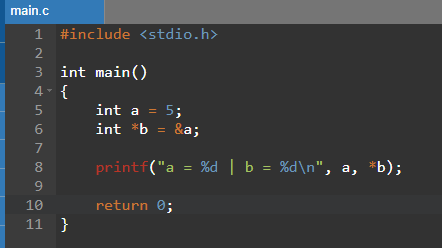
\includegraphics[width=7cm,height=4cm,keepaspectratio=false]{imagens/ponteiro.png}
		
	\end{figure}
	
	Acima, o que acontece é que:
	
	\begin{itemize}
		\item int a = 15; -> Você está colocando o valor 15 dentro da variável a.
	\end{itemize}
	
	\chapter{Falando de funções}
	
	
	
	

\end{document}

